\documentclass[UTF8]{ctexart}
    \title{\huge Destroyer2D Documentation}
    \author{\large 2015011308 唐适之}
    \date{}
    \usepackage[top=1in, bottom=1in, left=1.25in, right=1.25in]{geometry}
    \usepackage{enumitem}
	\usepackage{graphicx}
    \renewcommand{\figurename}{Figure}
    \renewcommand{\contentsname}{Contents}

\begin{document}
    
    \maketitle

    \tableofcontents

    \section{Introduction}

        Destroyer2D is a game. The players' aim is to build a ship or other types of structures, and move to the destination under bad sea conditions and enemies' attack.

        Destroyer2D makes use of \textit{LiquidFun} to provide 2D physics simulation, and \textit{GLFW} to load \textit{OpenGL} on different platforms (\textit{OpenGL} provides GUI rendering). All others including gaming workflow control, human interface, game items design, etc, are done by Destroyer2D.

    \section{Building}

        This section will describe how to build \textit{Destroyer2D}. Please notice that, Destroyer2D won't be built on a \textbf{virtual machine}, unless there is an OpenGL with high enough version. Most virtual machines provide poor OpenGL support.

        \subsection{Dependencies}

            Both of \textit{LiquidFun} and \textit{GLFW} are included in the \textit{third\_party} directory, so you don't have to install them by yourself. But you have to install \textbf{their} dependencies as listed below:

            \noindent \textbf{\textit{For Linux}}

            \begin{itemize}
                \item cmake (>= 2.8.12.1)
                \item OpenGL: libglapi-mesa (>= 8.0.4)
                \item Xlib: libx11-dev
                \item libXi: libxi-dev
                \item xorg-dev
                \item libgl1-mesa-dev
            \end{itemize}

            If you use \textit{apt-get}, just type

            \begin{verbatim} sudo apt-get install cmake libglapi-mesa libx11-dev libxi-dev xorg-dev libgl1-mesa-dev \end{verbatim}

            \noindent \textbf{\textit{For Windows}}

            \begin{itemize}
                \item cmake (>= 2.8.12.1)
                \item Windows (>= 7)
                \item Visual Studio (2010 or 2012)
            \end{itemize}

            They can be downloaded from their official sites.

        \subsection{Building}

            \noindent \textbf{\textit{For Linux}}

            Execute

            \begin{verbatim}cmake .
make \end{verbatim}

            You will get executable \textit{bin/Destroyer2D}.

            If you want to build in Debug mode, execute

            \begin{verbatim}cmake -DCMAKE_BUILD_TYPE=Debug
make \end{verbatim}

            If you want to switch back to Release mode, execute

            \begin{verbatim}cmake -DCMAKE_BUILD_TYPE=Release
make \end{verbatim}

            \noindent \textbf{\textit{For Windows}}

            You can use CLI cmake command as below:

            For Visual Studio 2012, execute

            \begin{verbatim}cmake -G "Visual Studio 11" \end{verbatim}

            For Visual Studio 2010, execute

            \begin{verbatim}cmake -G "Visual Studio 10" \end{verbatim}

            If you run cmake under Cygwin, you need to unset temp variables as

            \begin{verbatim}( unset {temp,tmp,TEMP,TMP} ; cmake -G "Visual Studio 11" ) \end{verbatim}

            or

            \begin{verbatim}( unset {temp,tmp,TEMP,TMP} ; cmake -G "Visual Studio 10" ) \end{verbatim}

            You can also use cmake GUI interface, but remember to choose Release mode, or it will be very slow.

            \textbf{Then}, double-click on \textit{Destroyer2D.sln} to open the solution. Select \textit{Build -> Build Solution} from the menu.

            You will get executable \textit{bin/Release/Destroyer2D}.

            You can perform a Debug build as described in Linux section, or use GUI to select Debug, but you should fully clean the binaries built previously.

            \noindent \textbf{\textit{For OS X}}

            Unfortunately, there is a known issue about rendering textures with OpenGL on OS X, so building on OS X is not supported.

    \section{Usage}

        This section will describe how to play this game.

        First, a player will enter the building scene. He or she can pick materials from the left, which are:

        \begin{itemize}
            \item Small Wooden Block
            \item Large Wooden Block -- These blocks can be used as scaffolding.
            \item Small Engine
            \item Large Engine -- These engines are used to provide force.
            \item Steel Ball
            \item Bomb -- A bomb can be ignited manually or in a crash. It can destroy items.
            \item Steel Stick
            \item Wooden Stick -- Sticks can be used to connect things together.
        \end{itemize}

        Click on the material to get one of them, and click again on the space to put it down. Click on the right button to cancel this putting process. For sticks, the player can draw lines with the cursor to connect things together. If the player place an engine or a bomb, he or she can choose LETTER key to control it. For example, choose key 'A' to start an engine or ignite a bomb. Moreover, the button with a red cross on the lower-left can be used to delete objects. The player can also drag things with the cursor.

        Note that different materials have different properties. Apparently steel is much heavier than wood, and is harder. When crash happens, things may be damaged. However, it's not apparently that a single flying steel stick has more probability to be damaged than a wooden block, because it have more momentum. Players should also pay attention to the shape of what he or she builds, because the shape of an objects in water is more important in 2D world than 3D. If finding unable to build a complex structure, using wooden block as scaffolding is suggested.

        Click LAUNCH button to battle. The structure built will be saved to file, so it can be improved again if failing the battle. In battle, use the key the player set before to control the movement. Move to the right most site across the red line to win the game. The distance that have to move through is approximately five times the width of the building area. If feeling despaired to win, for example in the situation of looseing your engine, click the red cross on the upper-left to go back to building scene.

        Currently there are 3 level: 0, 1, 2. When the player win in one level, he or she will enter the next. He or she can improve on the structure and battle again. However, if closing the game, the player will go back to level 0.

    \section{System Architecture}

        \subsection{Main Workflow}

            \textit{Destroyer2D} runs step by step, i.e. there is a main loop that continuously repeats. In each step, data are updated by gaming control and physical simulation and finally passed to the next step.

            There are 3 classes that play as the skeleton of the main loop as three levels: \textit{Window}, \textit{World}, and \textit{MainWorld}. \textit{Window::run()}, \textit{World::step()} and \textit{MainWorld::step()} are directly components of the main loop. Class \textit{Window} handles I/O with \textit{GLFW}, i.e. sends the rendered images and retrieve user inputs. It is the most basic level. \textit{World} maintains a generic playing scene, which can be extended to more than one type of game. It handles the inputs, renders the items and call \textit{LiquidFun} to do the simulation. And it is the intermediate level. \textit{MainWorld} inherits from \textit{World} and extends it to be a specific game, i.e. players build structure and battle. It handles the more specific gaming control and is the top level.

            The whole picture of the main loop is depicted on the diagram below. 

            \begin{figure}[htp]
                \makebox[\textwidth][c]{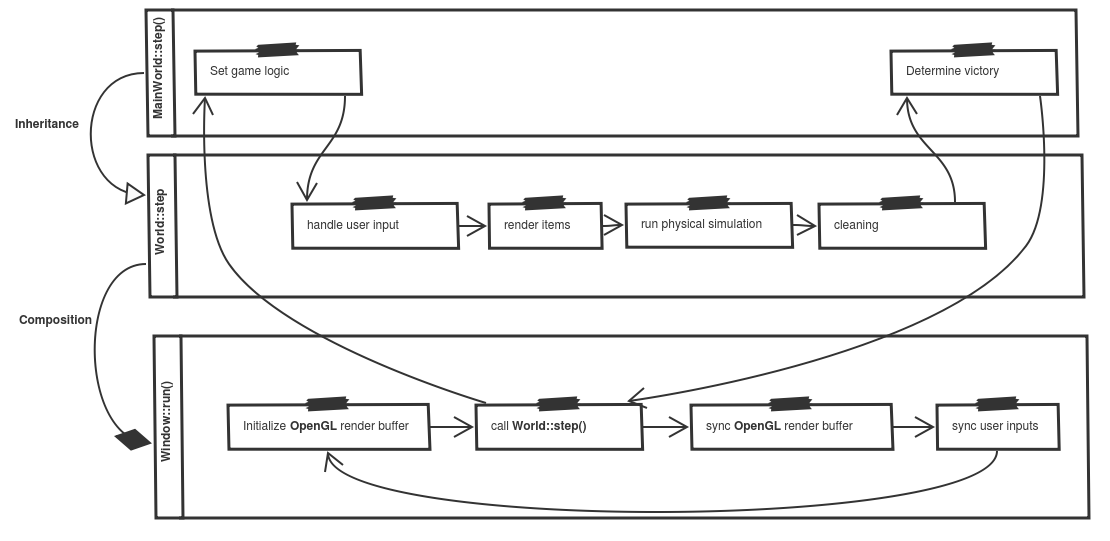
\includegraphics[width=1.3\textwidth]{mainloop.png}}
                \caption{Main Loop}
            \end{figure}

        \subsection{Subroutines}

            There are several subroutines in the main loop, some of which are relatively complex and are described below.

            User inputs include keyboard input and mouse input. Raw data can be retrieve from \textit{GLFW}. Keyboard input is relatively simple, so it can be handled directly in class \textit{World}. Mouse input includes clicking buttons, clicking to put items, dragging items, etc. Class \textit{MouseCallback} and its derived class are a polymorphism used to set specify changes accroding to the input. These classes are registered to class \textit{MouseHandler} as observers, and \textit{MouseHandler} preprocess the mouse input and call those observers. It is depicted as the diagram \textit{MouseHandler} below.

            \begin{figure}[htp]
                \centering
                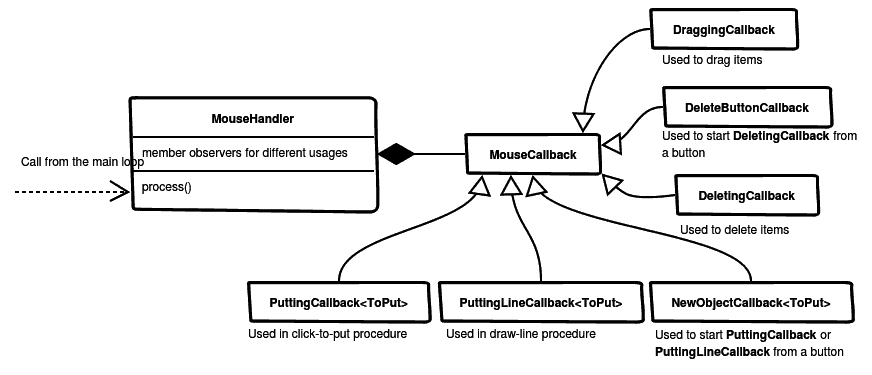
\includegraphics[width=\textwidth]{mousehandler.png}
                \caption{MouseHandler}
            \end{figure}

            Every body or particle system object in \textit{LiquidFun} are connected with one \textit{Matter} object in \textit{Destroyer2D}. Data and strategies used in physical simulations, rendering, and gamming controls are all defined in these class. Several items are similar, so they are grouped together. Therefore, \textit{Matter}'s polymorphism hierarchy is well organized. It is shown in the diagram \textit{Matter} below.

            \begin{figure}[htp]
                \centering
                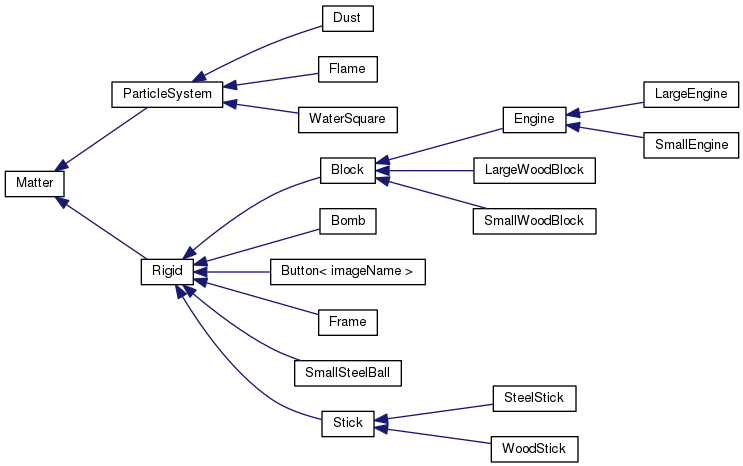
\includegraphics[width=\textwidth]{matter.png}
                \caption{Matter}
            \end{figure}

            Class \textit{Render} takes charge of rendering items into images using \textit{OpenGL} API. It can be divided into three major parts.

            \begin{enumerate}
                \item Rendering particle systems. Particle systems especially water needs special rendering technique to display a smooth appearance. \textit{Destroyer2D} first renders water particles into circles with gradient transparency into a buffer, then renders it again with a transparency threshold from the buffer onto the screen.
                \item Rendering items. There are 4 shapes can be used in \textit{LiquidFun}: polygon, circle, edge and chain. Currently only polygon and circle are used, and items in circle shapes are rendered as 36-gons. But for further extendence, a base class stub \textit{Render::FixtureRenderer} is preserved and it has only one subclass \textit{Render::PolygonRenderer}.
                \item Rendering other UI components. Other UI components including pictures and texts are rendered in class \textit{Render} for \textit{OpenGL} doesn't provide open-use functions to render them.
            \end{enumerate}

    \section{Detailed Reference}

        Further reference to each class and function in the project can be found in \textit{doc/reference/html/index.html}, which is generated by \textit{Doxygen}.

\end{document}
